\documentclass[12pt]{article}
\usepackage{graphicx, subfigure}

\begin{document}

\title{An Example of Augmenting a Latin Hypercube}
\author{Rob Carnell}
% Remove command to get current date 
\date{21 October 2006}
\maketitle

Suppose that a computer simulation study is being designed that requires expensive runs.  A Latin hypercube design is desired for this simulation so that the expectation of the simulation output can be estimated efficiently given the distributions of the input variables.  Latin hypercubes are most often used in highly dimensional problems, but the example shown is of small dimension.  Suppose further that the total extent of funding is uncertain.  Enough money is available for 5 runs, and there is a chance that there will be enough for 5 more.  However, if the money for the additional 5 runs does not materialize, then the first 5 runs must be a Latin hypercube alone.  A design for this situation can be created using the \texttt{lhs} package.\\

First create a random Latin hypercube using the \texttt{randomLHS(n, k)} command:\\
\\
\indent\indent{\texttt{> A <- randomLHS(5,2)}}\\
\\
An example of this hypercube is shown in Figure \ref{fig:original5}.  Note that the $Latin$ property of the hypercube requires that each of the 5 equal probability intervals be filled (i.e. each row and each column is filled with one point).  Also notice that the exact location of the design point is randomly sampled from within that cell using a uniform distribution for each marginal variable.\\


\begin{figure}[p]
	\centering
		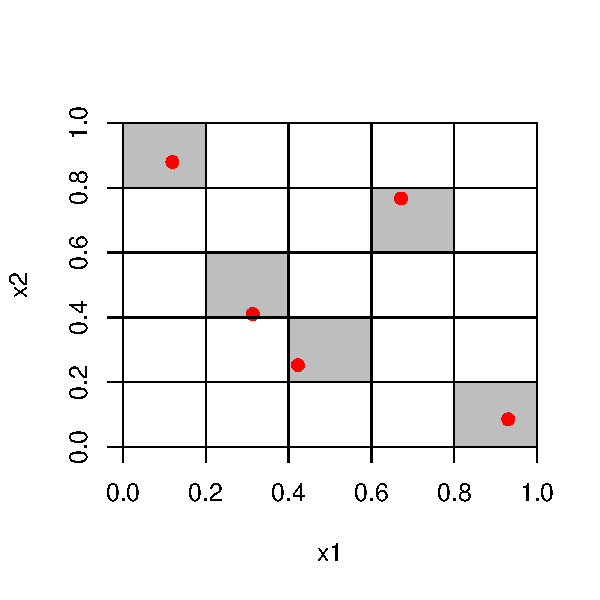
\includegraphics{original5.pdf}
	  \caption{A randomly produced Latin Hypercube with uniform marginal distributions for 2 parameters with 5 simulations.}
	\label{fig:original5}
\end{figure}

Next, in order to augment the design with more points use \texttt{augmentLHS(lhs, m)}.  The following will add 5 more points to the design:\\
\\
\indent\indent{\texttt{> B <- augmentLHS(A, 5)}}\\
\\
The \texttt{augmentLHS} function works by re-dividing the original design into $n+m$ intervals (e.g. 5+5=10) keeping the original design points exactly in the same position.  It then randomly fills the empty row-column sets.  The results are shown in Figure \ref{fig:augmented10}.

\begin{figure}[p]
	\centering
		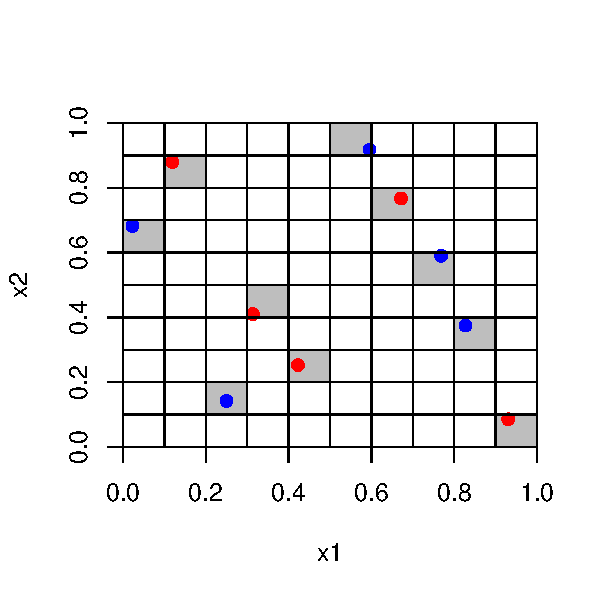
\includegraphics{augmented5.pdf}
	  \caption{A randomly produced Latin Hypercube of 5 points (red) with 5 augmented points (blue).  Each parameters has a uniform marginal distributions.}
	\label{fig:augmented10}
\end{figure}

The \texttt{augmentLHS} function uses the following algorithm (see the documentation for \texttt{augmentLHS}):
\begin{itemize}
	\item Create a new $(n+m)$ by $k$ matrix to hold the candidate points after the design has
been re-partitioned into $(n+m)^{2}$ cells, where $n$ is number of
points in the original $lhs$ matrix.\\
  \item Then randomly sweep through each
column (1\ldots$k$) in the repartitioned design to find the missing cells.\\
  \item For each column (variable), randomly search for an empty row, generate a
random value that fits in that row, record the value in the new matrix.
The new matrix can contain more than $m$ points unless $m = 2n$,
in which case the new matrix will contain exactly $m$ filled rows.\\
  \item Finally, keep only the first $m$ rows of the new matrix.  It is guaranteed that there
will be $m$ full rows (points) in the new matrix.  The deleted rows are partially full.
The additional candidate points are selected randomly because of the random search
used to find empty cells.\\
\end{itemize}
  
Also notice that because the original points are randomly placed within the cells, depending on how you bin the marginal distributions, a histogram (of x1 for example) will not necessarily be exactly uniform.\\

Now, the augmenting points do not necessarily form a Latin Hypercube themselves.  The original design and augmenting points may form a Latin Hypercube, or there may be more than one point per row in the augmented design.  If the augmented points are equal to the number of original points, then a strictly uniform Latin hypercube is guaranteed.  An example of an augmented design which is not uniform in the marginal distributions is given in Figure \ref{fig:badAugment}.  The commands were:\\
\\
\indent\indent{\texttt{> A <- randomLHS(7, 2)}}\\
\indent\indent{\texttt{> B <- augmentLHS(A, 3)}}\\
\\

\begin{figure}[p]
  \centering
  \subfigure[Original design with 7 points.]{
    \label{fig:badAugment:a} %% label for first subfigure
    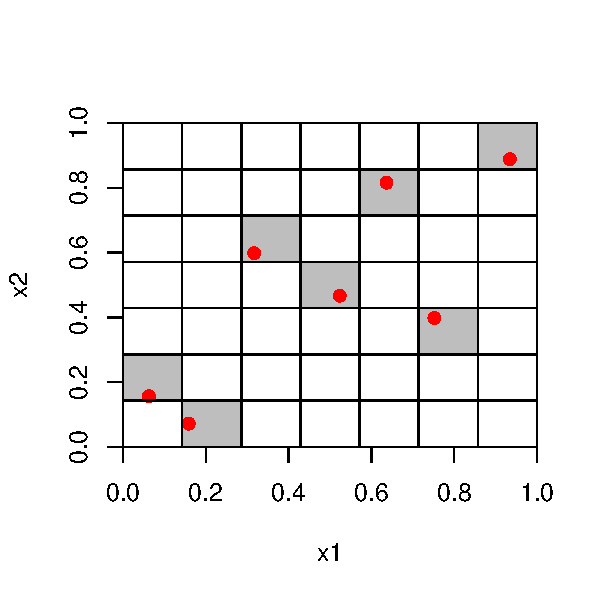
\includegraphics[width=3.0in]{original7.pdf}
  }
  \hspace{0.5in}
  \subfigure[Augmented design with 3 additional points.  Note that row 9 has 2 points and row 3 has none.]{
    \label{fig:badAugment:b} %% label for second subfigure
    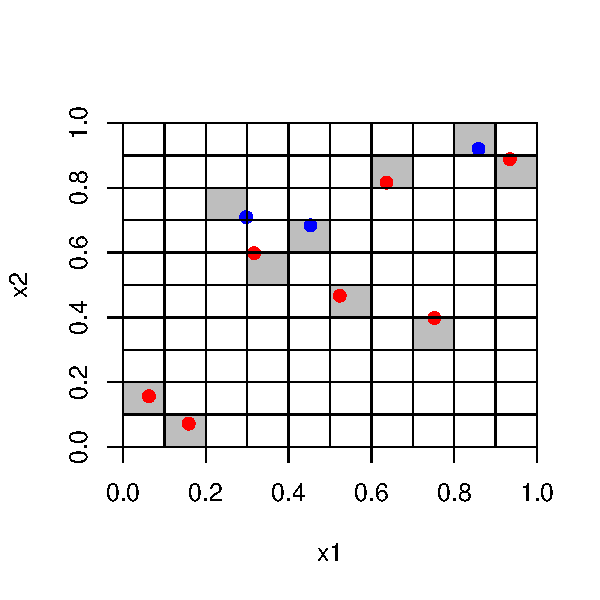
\includegraphics[width=3.0in]{augmented3.pdf}
  }
  \caption{Augmented Latin hypercube design with a non-uniform marginal distribution.}
  \label{fig:badAugment} %% label for entire figure
\end{figure}

\end{document}
